% !TEX root = catron-dissertation.tex
\epstopdfsetup{outdir=./images/07_multiple_sensor_filtering/}

\chapter{Multiple Sensor Filtering Techniques}
\label{chap:07_multiple_filter}

The previous chapter investigated filtering optical wavefront corruption by applying a variety of filters to the wavefront in the multi-dimensional spectral domain.
These techniques involve only data from the optical wavefront itself and user knowledge and experience to obtain filtered data.
When additional data streams are available, such as from microphones or accelerators, a targeted filter mechanisms become available.


A previous study \cite{DeLucca-2014-RAJvGdv7} focused on using the combination of linear stochastic estimation (LSE) and spectral proper orthogonal decomposition (SPOD) to remove vibration related contamination from aero-optical wind-tunnel measurements.
This process along with optical tip and tilt removal showed approximately an 85\% reduction in the measured $\opdrms$ by combining accelerator measurements with optical wavefront measurements.

\section{Optical Tip and Tilt}
Zernike polynomials are traditionally used for describing optical aberrations of a optical system \cite{Born-1965-HHGYgjdH}.
These polynomials are defined on the unit circle and form a set of orthogonal functions,
\begin{equation}
  Z_n^m(\rho,\theta) = R_n^m(\rho)\cos(m\theta)
  \label{eqn:07_zernike}
\end{equation}
where $R_n^m(\rho)$ is the radial basis function and $\cos(m\theta)$ is the angular basis function.
For values of $-m$ the angular basis function becomes $\sin(m\theta)$.
The radial basis function are developed from Jacobi polynomials but for purposes in this study, only a few simple ones will be used.
An optical wavefront can be approximated by a summation of Zernike polynomials multiplied by their corresponding coefficients
\begin{equation}
  \wf \approx \sum Z_ja_j \textrm{.}
  \label{eqn:07_zernike_coeff}
\end{equation}

The Noll naming scheme is an method of organizing the Zernike polynomials into a single notation of $Z_j$, along with normalizing each polynomial to have a spatial RMS equal to one \cite{Noll-1976-HHKzd88f}.
The first three of these using the Noll naming scheme are piston, tip, and tilt.
Piston is simply the average $\opd$ value of the single wavefront frame
\begin{equation}
  Z_1 = 1 \textrm{.}
  \label{eqn:07_zernike_1}
\end{equation}
Tip and tilt are the best planar fit to the $\opd$ along the x-axis and y-axis respectively where tip is
\begin{equation}
  Z_2 = 2\rho\cos\theta \textrm{,}
  \label{eqn:07_zernike_2}
\end{equation}
and tilt is
\begin{equation}
  Z_3 = 2\rho\sin\theta \textrm{.}
  \label{eqn:07_zernike_3}
\end{equation}
Once the coefficients for these modes are solved for they can be filtered out
\begin{equation}
  WF^F = WF-\sum Z_ja_j \textrm{.}
\end{equation}

\section{LSE-SPOD}
The LSE-SPOD technique starts with performing SPOD on the primary data set and then using the Fourier transforms of the additional sensor data to perform a filtering operation.
The spectral proper orthogonal decomposition technique is described in detail by Schmidt and Colonius \cite{Schmidt-2020-m2emACkX}.
A schematic of the SPOD algorithm is shown in Figure \ref{fig:07_spod_algorithm}.
\begin{figure}
  \centering
  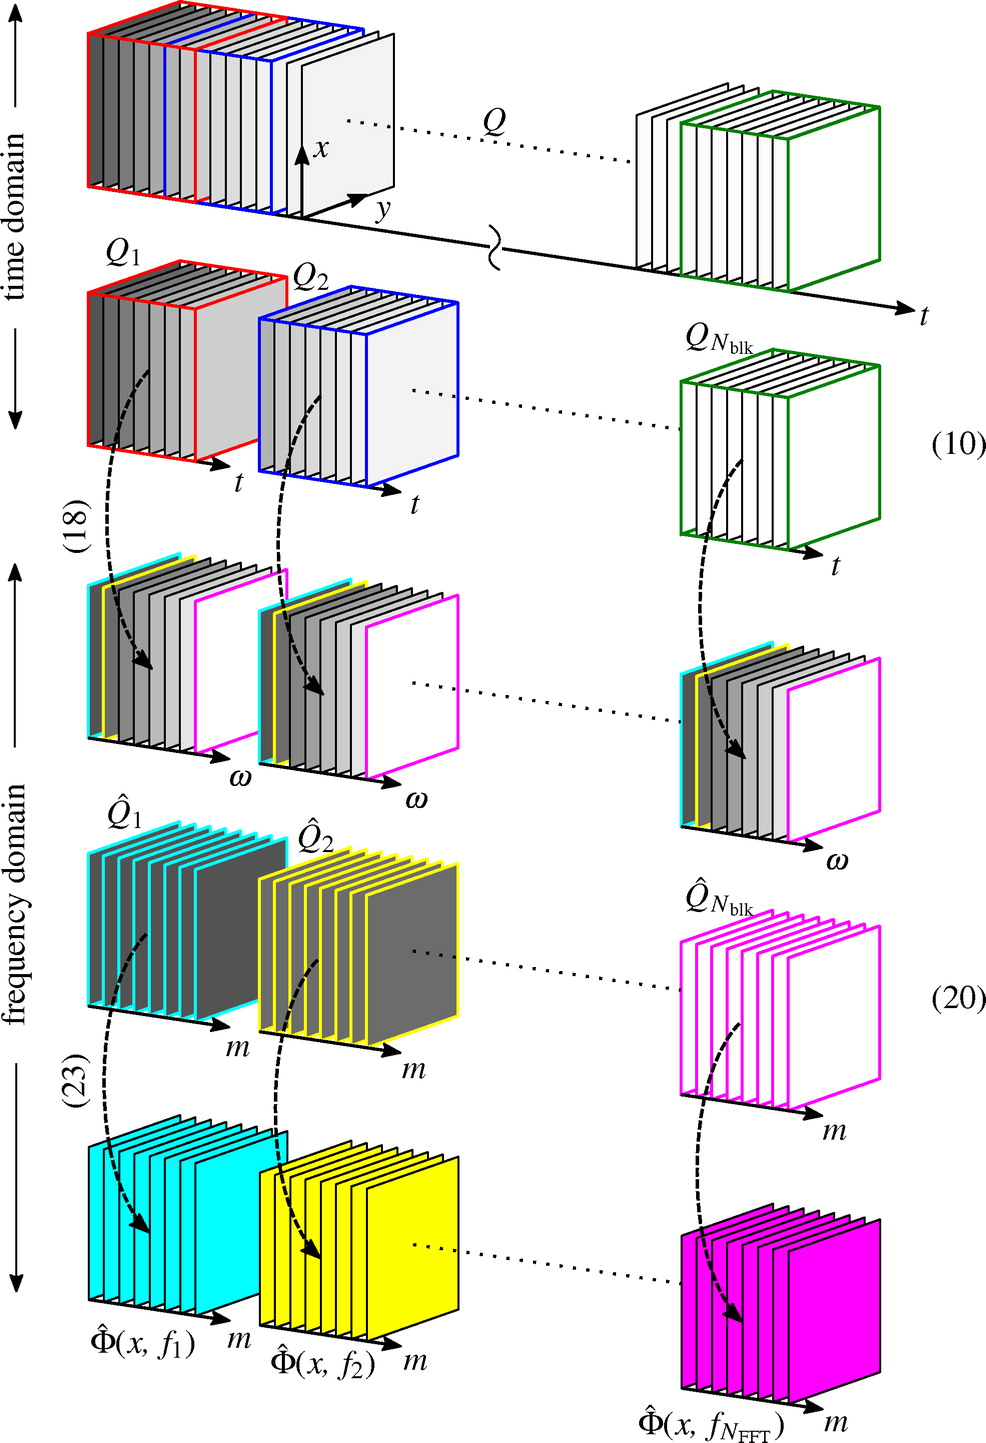
\includegraphics{../other-sources/schmidt_2020_figure_01.jpeg}
  \put(-20,235){\fcolorbox{white}{white}{\footnotesize(\ref{eqn:07_data_block})}}
  \put(-230,210){\rotatebox{90}{\fcolorbox{white}{white}{\color{white}{empt}}}}
  \put(-20,102){\fcolorbox{white}{white}{\footnotesize(\ref{eqn:07_frequency_block})}}
  \put(-231,69){\rotatebox{90}{\fcolorbox{white}{white}{\footnotesize(\ref{eqn:07_pod_01}-\ref{eqn:07_pod_04})}}}
  \caption{Schematic of the SPOD algorithm (taken from \cite{Schmidt-2020-m2emACkX}). The numbers in parentheses denote the equations used.}
  \label{fig:07_spod_algorithm}
\end{figure}
The algorithm begins by separating the original data set, $Q$, into a number of smaller blocks,
\begin{equation}
  Q = \left[
  \begin{matrix}
    \mid & \mid & & \mid \\
    q^{(1)} & q^{(2)} & \cdots & q^{(N)} \\
    \mid & \mid & & \mid
  \end{matrix}
  \right]\textrm{,}\quad Q\in\mathbb{C}^{M\times N}
  \label{eqn:07_data_block}
\end{equation}
where $M$ is the total number of degrees of freedom (number of spatial points times the block length in time) and $N$ is the number of blocks.
Each block is then Fourier Transformed in the temporal dimension or through all dimensions.
Once in the frequency domain the data blocks are then reorganized by creating new blocks of identical temporal-frequencies,
\begin{equation}
  \hat{Q} = \left[
  \begin{matrix}
    \mid & \mid & & \mid \\
    \hat{q}^{(1)} & \hat{q}^{(2)} & \cdots & \hat{q}^{(N)} \\
    \mid & \mid & & \mid
  \end{matrix}
  \right]\textrm{,}\quad \hat{Q}\in\mathbb{C}^{M\times N}
  \label{eqn:07_frequency_block}
\end{equation}
where $M$ is now the number of spatial points times the number of blocks and $N$ is block length in time.
Proper orthogonal decomposition is then performed separately on each temporal-frequency block via either traditional POD
\begin{equation}
  \hat{C} = \frac{1}{N-1}\hat{Q}\hat{Q}^H \textrm{,}
  \label{eqn:07_pod_01}
\end{equation}
\begin{equation}
  \hat{C}W\hat{\Phi}=\hat{\Phi}\hat{\Lambda} \textrm{,}
  \label{eqn:07_pod_02}
\end{equation}
or the method of snapshots,
\begin{equation}
  \hat{Q}^HW\hat{Q}\hat{\Psi}=\hat{\Psi}\hat{\Lambda} \textrm{,}
  \label{eqn:07_pod_03}
\end{equation}
\begin{equation}
  \hat{\Phi}=\hat{Q}\hat{\Psi} \textrm{,}
  \label{eqn:07_pod_04}
\end{equation}
where $H$ denotes the Hermitian transpose, $W$ is a weighting matrix, $\Phi$ is the set of deterministic spatial functions, $\Lambda$ is the eigen-values, and $\Psi$ is the coefficient matrix.

The linear stochastic estimation portion of the technique is described by Adrian \cite{Adrian-1975-VenaZyuv}.
This process uses a linear sum, $L_{ij}$, of additional measurements, $y_j$, to approximate a measured signal, $x_i$,
\begin{equation}
  x_i^{LSE}=L_{ij}y_j \textrm{,}
  \label{eqn:07_lse_01}
\end{equation}
where
\begin{equation}
  L_{ij} = \langle x_iy_k\rangle\langle y_jy_k\rangle^{-1} \textrm{.}
  \label{eqn:07_lse_02}
\end{equation}
When combined with SPOD, the estimation matrix, $L$, becomes
\begin{equation}
  L=(\hat{\Psi}\hat{y}^H)(\hat{y}\hat{y}^H)^{-1} \textrm{,}
  \label{eqn:07_lse_spod_01}
\end{equation}
which allows for an estimated version of the coefficient matrix to be calculated
\begin{equation}
  \hat{\Psi}^E=L\hat{y} \textrm{.}
  \label{eqn:07_lse_spod_02}
\end{equation}
The estimated coefficient matrix contains portions of the original signal that best resemble the additional sensor data.
Assuming that the additional sensor data represents signal contamination of the original signal, a filtered coefficient matrix can be computed from the difference between the original and estimated coefficient matrix.
\begin{equation}
  \hat{\Psi}^F=\hat{\Psi}-\hat{\Psi}^E \textrm{.}
  \label{eqn:07_lse_spod_03}
\end{equation}
A filtered signal, $Q^F$ can be constructed by using the filtered coefficient matrix and the spatial functions,
\begin{equation}
  \hat{Q} = \hat{\Psi}^F\hat{\Phi}^H \textrm{.}
\end{equation}

\section{Filtering Experimental Data}




\begin{figure}
  \centering
  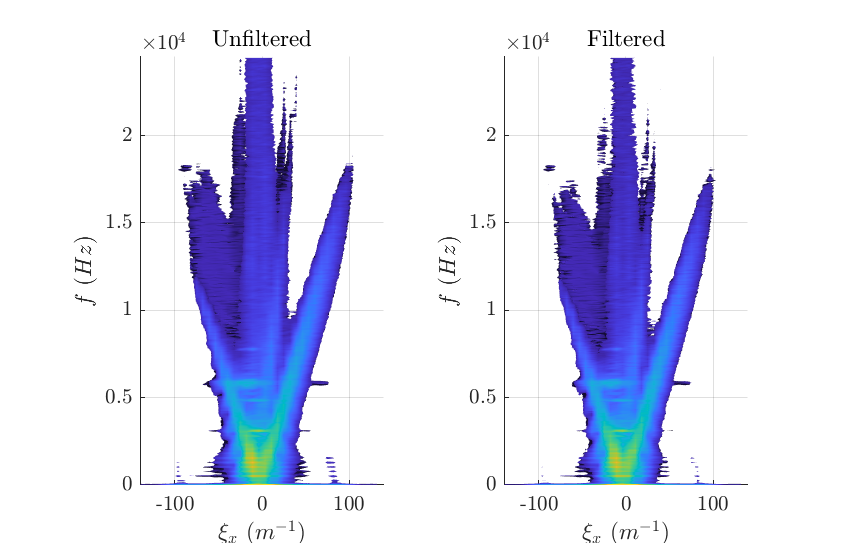
\includegraphics{../matlab/07_multiple_sensor_filtering/lse_mspod.eps}
  \caption{REPLACE}
  \label{fig:07_lse_mspod}
\end{figure}



\begin{table}
  \centering
  \caption{REPLACE}
  \input{../matlab/07_multiple_sensor_filtering/lse_mspod_table.txt}
  \label{tab:07_lse_mspod_table}
\end{table}
